% Wei-Jin Huang -- academic CV  (violet banner edition)
% Build: xelatex wei_jin_huang_cv.tex
\documentclass[10pt,a4paper]{article}

\usepackage[a4paper,top=1.0cm,bottom=0.8cm,left=1.45cm,right=1.45cm]{geometry}
\usepackage{fontspec}
\usepackage{microtype}
\usepackage{xcolor}
\usepackage{graphicx}
\usepackage{enumitem}
\usepackage{ragged2e}
\usepackage{fontawesome5}
\usepackage{tikz}
\usepackage[hidelinks]{hyperref}

% ---- fonts -----------------------------------------------------------------
\setmainfont{HelveticaNeueLTPro-Roman.otf}[
  Path = fonts/,
  BoldFont = HelveticaNeueLTPro-Md.otf,
  ItalicFont = HelveticaNeueLTPro-Roman.otf,
]

% ---- palette ---------------------------------------------------------------
\definecolor{ink}{HTML}{1F2430}      % body text
\definecolor{muted}{HTML}{6B7280}    % secondary text
\definecolor{primary}{HTML}{6D28D9}  % deep violet  (titles, name highlight)
\definecolor{banner}{HTML}{5B21B6}   % banner background
\definecolor{accent}{HTML}{DB2777}   % magenta      (dates, venues, bars)
\definecolor{rule}{HTML}{E3DCF2}     % light violet rule
\definecolor{bsub}{HTML}{E9D5FF}     % banner subtitle (violet-200)
\color{ink}

\hypersetup{colorlinks=true,urlcolor=primary,linkcolor=primary}
\setlength{\parindent}{0pt}
\pagestyle{empty}
\linespread{0.93}

% ---- helpers ---------------------------------------------------------------
% section heading: magenta bar + violet title + thin rule
\newcommand{\cvsection}[1]{%
  \vspace{2pt}\par\noindent
  {\color{accent}\rule[-1pt]{3.2pt}{12pt}}\hspace{6pt}%
  {\bfseries\large\color{primary}#1}\par
  \vspace{2.5pt}{\color{rule}\hrule height 1pt}\vspace{4pt}}

\newcommand{\dt}[1]{{\bfseries\color{accent}\footnotesize #1}}
\newcommand{\me}[1]{{\bfseries\color{primary}#1}}        % highlight my name
\newcommand{\venue}[2]{{\bfseries\color{accent}#1}\,{\color{muted}\footnotesize #2}}

% numbered badge for publications
\newcommand{\badge}[1]{%
  \tikz[baseline=(c.base)]{\node[fill=primary,text=white,rounded corners=2.5pt,
    inner xsep=0pt,inner ysep=0pt,minimum width=1.45em,minimum height=1.45em,
    font=\bfseries\small](c){#1};}}

% publication block: number / title / authors / venue / abstract / url
\newcommand{\pub}[6]{%
  \noindent
  \begin{minipage}[t]{1.55em}\vspace{1.5pt}\badge{#1}\end{minipage}\hspace{0.6em}%
  \begin{minipage}[t]{\dimexpr\linewidth-2.15em\relax}\vspace{0pt}
    \href{#6}{\bfseries\color{ink} #2}\par
    {\footnotesize\color{muted}#3}\par
    \vspace{0.5pt}#4\par
    \vspace{1pt}{\color{ink}{\bfseries\color{primary}Abstract:} #5}\par
  \end{minipage}\par\vspace{2.5pt}}

\begin{document}
\RaggedRight

% ============================ HEADER =======================================
\begin{minipage}[b]{0.78\textwidth}
  {\fontsize{25}{28}\selectfont\bfseries\color{primary} Wei-Jin Huang}\\[4pt]
  {\bfseries\color{accent} Ph.D. Student}{\color{muted}, Computer Science and Technology}\\[1.5pt]
  {\color{muted} Sun Yat-sen University, Guangzhou, China}\\[5pt]
  {\footnotesize\color{primary}%
    \faEnvelope[regular]~\href{mailto:huangwj235@mail2.sysu.edu.cn}{huangwj235@mail2.sysu.edu.cn}\quad
    \faGlobe~\href{https://vkgo.github.io/}{vkgo.github.io}\\[2.5pt]
    \faGraduationCap~\href{https://scholar.google.com/citations?user=jMrU_JYAAAAJ}{Google Scholar}\quad
    \faGithub~\href{https://github.com/vkgo}{github.com/vkgo}\quad
    \faKaggle~\href{https://www.kaggle.com/carmencita}{carmencita}}
\end{minipage}\hfill
\begin{minipage}[b]{0.2\textwidth}
  \raggedleft
  {\setlength{\fboxsep}{0pt}\setlength{\fboxrule}{0.8pt}%
   \fcolorbox{rule}{white}{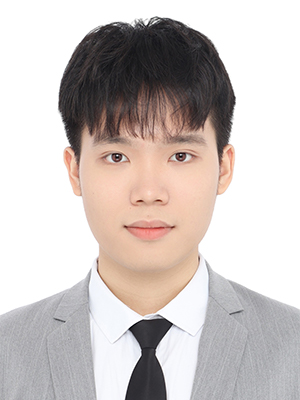
\includegraphics[height=2.85cm]{photo.jpg}}}
\end{minipage}

\vspace{6pt}
{\color{primary}\hrule height 1.5pt}
\vspace{2pt}

% ============================ SUMMARY ======================================
\cvsection{Research Summary}
I am a Ph.D.\ student at Sun Yat-sen University, advised by Prof.\ Wei-Shi Zheng, working on humanoid
learning and video action understanding. My research builds physically grounded systems that learn
whole-body human--humanoid interaction from human demonstrations and that understand fine-grained human
actions in video. I have published as (co-)first author at CVPR, ICCV, and ECCV, and I aim to advance
embodied intelligence through rigorous, impactful research.

% ============================ EDUCATION ====================================
\cvsection{Education}
{\bfseries Ph.D., Computer Science and Technology} -- Sun Yat-sen University (SYSU), Guangzhou, China \hfill \dt{2024.09 -- Present}\\
{\color{muted}\small Specialization: Humanoid Learning, Video Action Understanding}\\[2pt]
{\bfseries B.E., Network Engineering} -- South China University of Technology (SCUT), Guangzhou, China \hfill \dt{2020.09 -- 2024.07}\\
{\color{muted}\small Average grade ranking 3/66}

% ============================ PUBLICATIONS =================================
\cvsection{Selected Publications}
\pub
  {1}{Beyond Mimicry: Learning Whole-Body Human-Humanoid Interaction from Human-Human Demonstrations}
  {\me{Wei-Jin Huang}, Yue-Yi Zhang, Yi-Lin Wei, Zhi-Wei Xia, Juantao Tan, Yuan-Ming Li, Zhilin Zhao, Wei-Shi Zheng}
  {\venue{CVPR 2026}{- Proceedings of the Computer Vision and Pattern Recognition Conference}}
  {Physical human-humanoid interaction is hindered by scarce high-quality data. We leverage abundant human-human
   data via PAIR, a contact-preserving retargeting pipeline, and D-STAR, a hierarchical interaction policy that
   attains a state-of-the-art 75.4\% average success rate across six interactive tasks and transfers to a real
   Unitree G1 humanoid.}
  {https://cvpr.thecvf.com/virtual/2026/poster/37452}

\pub
  {2}{Modeling Multiple Normal Action Representations for Error Detection in Procedural Tasks}
  {\me{Wei-Jin Huang}, Yuan-Ming Li, Zhi-Wei Xia, Yu-Ming Tang, Kun-Yu Lin, Jian-Fang Hu, Wei-Shi Zheng}
  {\venue{CVPR 2025}{- Proceedings of the Computer Vision and Pattern Recognition Conference}}
  {Error detection in procedural activities is essential for AR-assisted and robotic systems, yet prior methods
   rely on temporal ordering or static prototypes of normal actions. We propose AMNAR, an Adaptive Multiple
   Normal Action Representation framework that predicts all valid next actions and reconstructs their normal
   representations for comparison with the ongoing action, setting state-of-the-art across EgoPER, HoloAssist,
   and CaptainCook4D (+7.4\% EDA / +6.5\% AUC over the prior best).}
  {https://openaccess.thecvf.com/content/CVPR2025/html/Huang_Modeling_Multiple_Normal_Action_Representations_for_Error_Detection_in_Procedural_CVPR_2025_paper.html}

\pub
  {3}{Less Static, More Private: Towards Transferable Privacy-Preserving Action Recognition by Generative Decoupled Learning}
  {Zhi-Wei Xia, Kun-Yu Lin, Yuan-Ming Li, \me{Wei-Jin Huang}, Xian-Tuo Tan, Wei-Shi Zheng}
  {\venue{ICCV 2025}{- Proceedings of the IEEE/CVF International Conference on Computer Vision}}
  {Privacy-preserving action recognition aims to protect individual privacy in action videos without compromising
   recognition, but existing methods struggle under video domain shifts. We propose GenPriv, a transferable
   framework that decouples static and dynamic video features and removes privacy-sensitive content from static
   features, achieving strong cross-domain action recognition while preserving privacy.}
  {https://openaccess.thecvf.com/content/ICCV2025/html/Xia_Less_Static_More_Private_Towards_Transferable_Privacy-Preserving_Action_Recognition_by_ICCV_2025_paper.html}

\pub
  {4}{EgoExo-Fitness: Towards Egocentric and Exocentric Full-Body Action Understanding}
  {Yuan-Ming Li, \me{Wei-Jin Huang (Co-First)}, An-Lan Wang, Ling-An Zeng, Jing-Ke Meng, Wei-Shi Zheng}
  {\venue{ECCV 2024}{- European Conference on Computer Vision}}
  {We present EgoExo-Fitness, a 32-hour full-body action understanding dataset of 1,276 cross-view fitness
   sequences from 40 subjects, captured by six synchronized egocentric and exocentric cameras. It is richly
   annotated with two-level temporal boundaries, natural-language comments, and 1-5 action-quality scores,
   enabling fine-grained interpretable action analysis beyond existing datasets.}
  {https://doi.org/10.1007/978-3-031-72661-3_21}

% ============================ INTERESTS ====================================
\cvsection{Research Interests}
{\bfseries\color{primary} Humanoid Learning:} embodied intelligence, whole-body control, imitation learning, human-humanoid
interaction; {\bfseries\color{primary} Video Understanding:} action recognition, temporal action understanding, video
representation learning

% ============================ EXPERIENCE ===================================
\cvsection{Experience}
{\bfseries Algorithm Engineer Intern} -- China Telecom (Tianyi Digital Life Technology) \hfill \dt{2023.03 -- 2023.05}
\begin{itemize}[leftmargin=1.2em,topsep=2pt,itemsep=1pt,parsep=0pt]
  \item Adapted the BEiT-3 multimodal foundation model to a real-world scene-classification task, raising
        accuracy from 93.1\% to 95.3\% via vision-language fine-tuning and task-specific data curation.
\end{itemize}

% ============================ HONORS =======================================
\cvsection{Honors and Awards}
\dt{2024}\hspace{0.7em}President Scholarship, Sun Yat-sen University (top 5\%)\\[2.5pt]
\dt{2022}\hspace{0.7em}Kaggle -- H\&M Personalized Fashion Recommendations, Silver (85/2952)\\[1.5pt]
\hspace*{2.05em}National Scholarship (1/66)\quad{\color{rule}\textbullet}\quad Tencent Scholarship -- First Class (1/66)\\[2.5pt]
\dt{2021}\hspace{0.7em}Kaggle -- G2Net Gravitational Wave Detection, Silver (57/1219)

\end{document}
